\documentclass{beamer}
\usepackage[utf8]{inputenc}

\usetheme{Madrid}
\usecolortheme{default}
\usepackage{amsmath,amssymb,amsfonts,amsthm}
\usepackage{txfonts}
\usepackage{tkz-euclide}
\usepackage{listings}
\usepackage{adjustbox}
\usepackage{array}
\usepackage{tabularx}
\usepackage{gvv}
\usepackage{lmodern}
\usepackage{circuitikz}
\usepackage{tikz}
\usepackage{graphicx}
\usepackage{mathtools}

\setbeamertemplate{page number in head/foot}[totalframenumber]

\usepackage{tcolorbox}
\tcbuselibrary{minted,breakable,xparse,skins}



\definecolor{bg}{gray}{0.95}
\DeclareTCBListing{mintedbox}{O{}m!O{}}{%
  breakable=true,
  listing engine=minted,
  listing only,
  minted language=#2,
  minted style=default,
  minted options={%
    linenos,
    gobble=0,
    breaklines=true,
    breakafter=,,
    fontsize=\small,
    numbersep=8pt,
    #1},
  boxsep=0pt,
  left skip=0pt,
  right skip=0pt,
  left=25pt,
  right=0pt,
  top=3pt,
  bottom=3pt,
  arc=5pt,
  leftrule=0pt,
  rightrule=0pt,
  bottomrule=2pt,
  toprule=2pt,
  colback=bg,
  colframe=orange!70,
  enhanced,
  overlay={%
    \begin{tcbclipinterior}
    \fill[orange!20!white] (frame.south west) rectangle ([xshift=20pt]frame.north west);
    \end{tcbclipinterior}},
  #3,
}
\lstset{
    language=C,
    basicstyle=\ttfamily\small,
    keywordstyle=\color{blue},
    stringstyle=\color{orange},
    commentstyle=\color{green!60!black},
    numbers=left,
    numberstyle=\tiny\color{gray},
    breaklines=true,
    showstringspaces=false,
}
\title{4.13.50}
\date{27th September, 2025}
\author{Puni Aditya - EE25BTECH11046}

\begin{document}

\frame{\titlepage}
\begin{frame}{Question}
Two equal sides of an isosceles triangle are given by the equations $7x - y + 3 = 0$ and $x + y - 3 = 0$ and its third side passes through the point $(1, -10)$. Determine the equation of the third side.
\end{frame}

\begin{frame}{Theoretical Solution}
Let the two equal sides of the isosceles triangle be represented by
\begin{align*}
    \vec{n_1}^\top\vec{x} &= c_1 \\
    \vec{n_2}^\top\vec{x} &= c_2
\end{align*}
and the third side by the line
\begin{align*}
    \vec{n}^\top\vec{x} &= c
\end{align*}
The third side of the isosceles, the base, is perpendicular to the angle bisector of the two equal sides.
\end{frame}

\begin{frame}{Theoretical Solution}
For a line passing through a given point $\vec{p}$,
\begin{align}
	\vec{n}^\top\vec{x} &= \vec{n}^\top\vec{p} \\
    \text{Here, }\vec{p} &= \myvec{1 \\ -10}
\end{align}
The third side of the isosceles, the base, is perpendicular to one of the angle bisector of the two equal sides and parallel to the other.
\begin{align}
    \vec{m_1} &= \frac{\vec{n_1}}{\norm{\vec{n_1}}} + \frac{\vec{n_2}}{\norm{\vec{n_2}}} \label{eq:31} \\
    \vec{m_2} &= \frac{\vec{n_1}}{\norm{\vec{n_1}}} - \frac{\vec{n_2}}{\norm{\vec{n_2}}} \label{eq:32}
\end{align}
\end{frame}

\begin{frame}{Theoretical Solution}
Hence,
\begin{align}
	\vec{n} = \vec{m_2}\text{ or }\vec{n} = \vec{m_1}
\end{align}
For the given question,
\begin{align}
    \vec{n_1} &= \myvec{7 \\ -1}\text{ and }\vec{n_2} = \myvec{1 \\ 1} \\
    \norm{\vec{n_1}} &= \sqrt{50} = 5\sqrt{2} \\
    \norm{\vec{n_2}} &= \sqrt{2}
\end{align}
\end{frame}

\begin{frame}{Theoretical Solution}
For the side parallel to $\vec{m_2}$, using \eqref{eq:31},
\begin{align}
    \vec{n} &= \frac{1}{5\sqrt{2}}\brak{\myvec{7 \\ -1} + \myvec{5 \\ 5}} = \frac{1}{5\sqrt{2}}\myvec{12 \\ 4} \\
    \vec{n} &= \myvec{3 \\ 1} \\
    \myvec{3 & 1}\vec{x} &= \myvec{3 & 1}\myvec{1 \\ -10} \\
	\myvec{3 & 1}\vec{x} &= -7
\end{align}
\end{frame}

\begin{frame}{Theoretical Solution}
For the side parallel to $\vec{m_1}$, using \eqref{eq:32},
\begin{align}    
    \vec{n} &= \frac{1}{5\sqrt{2}}\brak{\myvec{7 \\ -1} - \myvec{5 \\ 5}} = \frac{1}{5\sqrt{2}}\myvec{2 \\ -6} \\
    \vec{n} &= \myvec{1 \\ -3} \\
	\myvec{1 & -3}\vec{x} &= \myvec{1 & -3}\myvec{1 \\ -10} \\
    \myvec{1 & -3}\vec{x} &= 31
\end{align}
\end{frame}

\begin{frame}{Plot}
    \begin{figure}
        \centering
        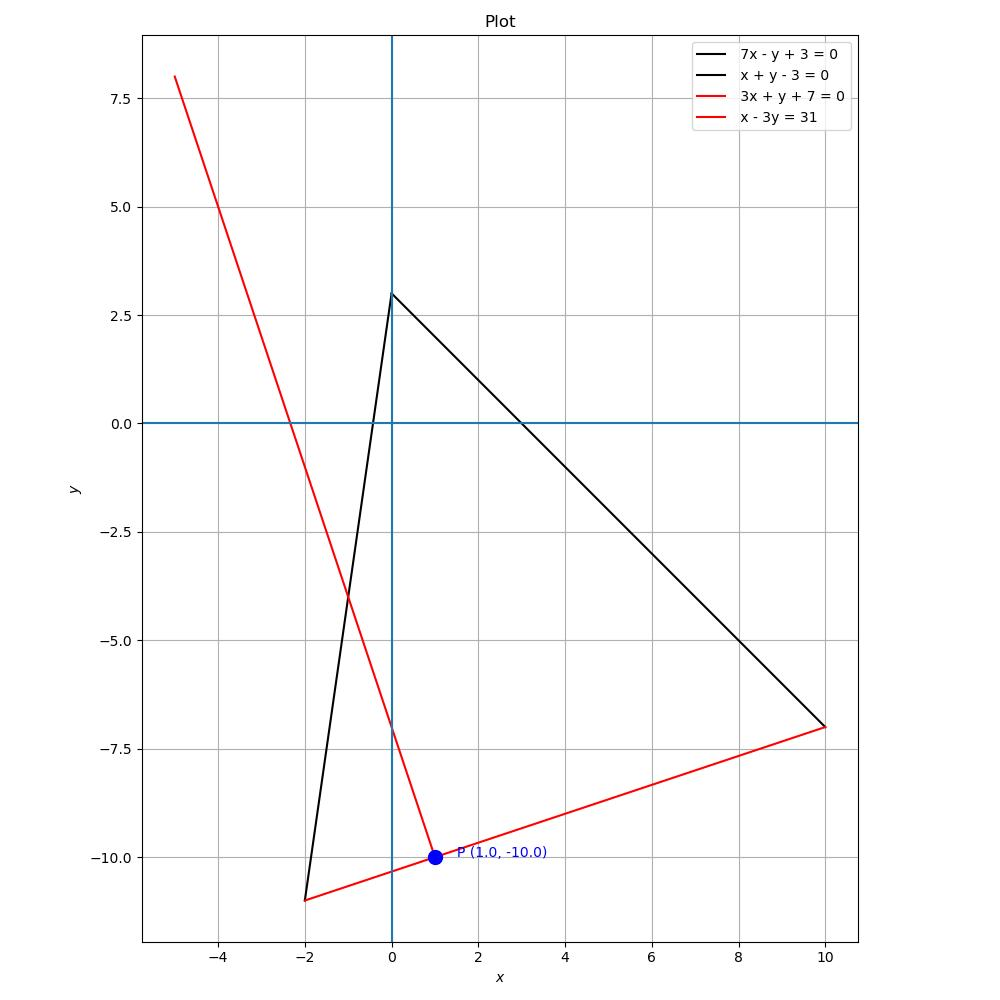
\includegraphics[width=0.5\columnwidth]{../figs/plot_c.jpg}
        \caption{Isosceles Triangle}
        \label{fig:fig}
    \end{figure}
\end{frame}

\end{document}
